%!TEX root = ../thesis.tex

\section{Speech representation learning paradigms} \label{sec:approach}
Due to the characteristics of speech, SSL pretext tasks developed for CV
and NLP may not directly apply to speech.
Below we summarize the characteristics of speech as compared to CV and NLP.
\begin{itemize}
\item \textit{Speech is a sequence.} 
Unlike CV, in which an image usually has a fixed size representation, it is
natural to represent a speech utterance as a variable-length sequence. 
Therefore, pretext tasks developed for CV cannot generally be directly
applied to speech.

\item \textit{Speech is a long sequence without segment boundaries.} 
Both text and speech can be represented as sequences. From this viewpoint, it
is natural to apply learning approaches developed for text directly to
speech. 
In NLP, morpheme-like tokens are widely used as sequence units in
pre-training. The standard BERT takes 512 morpheme-like tokens as
input, usually covering a paragraph including several sentences. 
However, speech signals consist of sound pressure measurements with thousands
of samples per second, resulting in sequences much longer than those for text. Even
spectral representations which reduce the sequence length can have hundreds of
frames per second.
Processing such sequences with typical neural network architectures like
Transformers can result in problems with running time and memory requirements. 
One could gather consecutive frames to form shorter segments,
but unlike text, there is no obvious segmentation for unlabeled
speech.
\item \textit{Speech is continuous.} 
In NLP, it is common to use a pretext task that models a categorical
distribution of masked or future inputs. Since text is easily broken down into
individual tokens such as words, subwords, or characters, it is
straightforward to define a finite vocabulary for such tasks.
However, this idea does not apply to speech modeling because speech
signals are continuous; 
in this sense there is no such thing as a speech vocabulary. 
\item \textit{Speech processing tasks are diverse.}
Building generalizable self-supervised representation models for diverse speech
processing tasks is challenging.
Speech contains rich, hierarchical information, and different speech tasks
may require mutually orthogonal information.
For example, speech recognition requires a model that extracts content information
but ignores speaker information; in contrast, speaker recognition 
requires a model that extracts speaker information but removes content information.
Therefore, it is challenging to define a self-supervised model whose
representations are suitable for both speech recognition and speaker
recognition. Analogous considerations apply within CV and NLP.
\end{itemize}

In the sections below, we group modern SSL pretext tasks designed for speech
into three main categories: \textit{generative} approaches,
\textit{contrastive} approaches and \textit{predictive} approaches. 
\Cref{fig:timeline} shows a timeline of the models covered in these sections
with each model colored according to our categorization. 
\Cref{table:pretext} summarizes model pretext tasks along within the categories.


\subsection{Notation}
\label{sec:notation}

To efficiently describe the different approaches, we use a simple
notation. Models are assumed to consist of functions $f(\cdot)$ and $g(\cdot)$, where $f(\cdot)$  denotes the representation model to be used after pre-training and $g(\cdot)$ is an auxiliary module needed only to support the pretext task. For instance, in a classic autoencoder, $f(\cdot)$ would denote the encoder and $g(\cdot)$ the decoder. For more complex models, these functions might consist of several components indicated by sub-indices $f_1(\cdot) \dots f_N(\cdot)$. As we will see, many self-supervised models use masking, which replaces some parts of the input or a hidden representation  by zeros or a learned vector. We use $m(\cdot)$ to denote a function that applies such masking to its input. Similar to $g(\cdot)$, this function is only used during pre-training. 

Given an acoustic input $X =\{x_1,x_2, ..., x_T\}$, $f(\cdot)$ outputs a representation $H =\{h_1,h_2,...,h_T\}$. The input~$X$ may be either the raw waveform samples or a sequence of spectral feature vectors. Both are viable options in practice. For simplicity, we do not distinguish between the two in our notation.  

While $f(\cdot)$ always takes an acoustic input, the input to $g(\cdot)$ can be either the acoustic signal or another learned representation. Most importantly, $g(\cdot)$ produces an output that is used for the pretext task but is not  used by $f(\cdot)$ to produce the representation $H$. Hence, $g(\cdot)$ can be discarded after pre-training. Finally, $f(\cdot)$ commonly downsamples the temporal dimension, but again, this is not crucial to understand the models, so consider only a single temporal scale $t\in\{1,\dots, T\}$ for notational convenience.

We use $Q = \{q_1,q_2, ..., q_T\}$ to denote representations that are quantized via codebook learning. Alternatively, discrete representations may take the form of one-hot vectors, or the equivalent integer IDs, which we denote by $C = \{c_1,c_2, ..., c_T\}$. We use a circumflex to denote that, for instance, $\hat{x}_t$ is an approximation of $x_t$. Finally, we often use a subscript when defining a loss, $\mathcal{L}_i$, to imply that the total loss is computed as a sum over $i$, unless otherwise stated.

For some models, we will refer to $H$ as a \emph{contextualized} representation which means that each $h_t$ is a function of some, linguistically speaking, long sub-sequence of $X$ spanning at least several phonemes. Usually, $h_t$ depends on the entire input $X$ or all previous timesteps $X_{[1,t]}$. In contrast, a \emph{localized} representation is one that only depends on a short part of the input $X_{[t - u,t + u]}$, where $u \geq 0$. The distinction between contextualized and localized may become fuzzy if $u$ is large, however, this is rarely the case.

\edit{After pre-training,} the representation model $f(\cdot)$ can be fine-tuned for a downstream task directly or used to extract features which are fed to another model, as visualized in \cref{fig:SSL_framework}. It is not uncommon to use the output representation~$H$, but often representations from hidden layers of $f(\cdot)$ are better suited \parencite{pasad_layerwise_2021}.


\begin{figure*}[t]
    \centering
    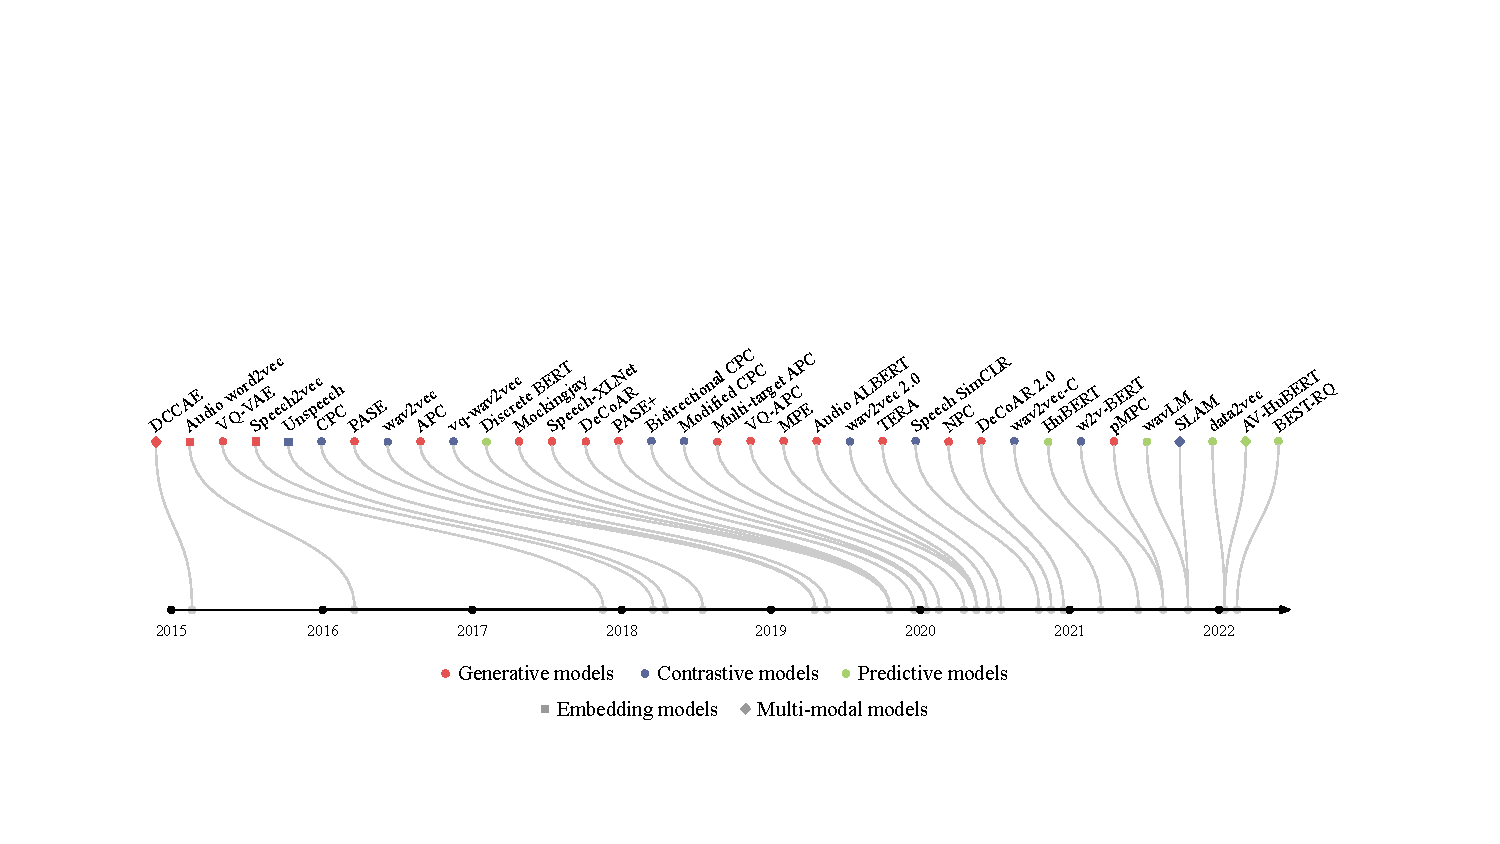
\includegraphics[width=0.98\textwidth]{paper_review/model_timeline.pdf}
   % \includegraphics[width=0.98\textwidth]{paper_review/model_timeline_wo_dccae.pdf}
	 \caption[Selection of self-supervised models for speech.]{A selection of models listed according to first publication date
	 on arXiv or conference submission date when this clearly precedes the
	 former. The models are categorized as generative, contrastive, or predictive.
	 In addition, some models are characterized as embedding models or
	 multi-modal models, although most learn frame-level
	 representations from speech only. Some models use a mixture of generative
	 and contrastive tasks. For instance, PASE and PASE+ use a multi-task setup,
	 but find that generative tasks are the most important for downstream
	 task performance~\parencite{pascual_learning_2019}.}
    \label{fig:timeline}
\end{figure*}


 

\subsection{Generative approaches}
\label{sec:generative}

\subsubsection{Motivation}

In this category, the pretext task is to generate, or reconstruct, the input data based on some limited view. This includes predicting future inputs from past inputs, masked from unmasked, or the original from some other corrupted view.  ``Generative'' as used in this paper hence refers to models that target the original input in their pretext task. Note that this differs from generative models, which learn \ci{distributions that allow} to sample new data.

\subsubsection{Approaches}

\paragraph{Autoencoding} 
Since their introduction in the mid-1990s~\parencite{hinton_autoencoders_1994}, autoencoders (AEs)
have played an essential role in learning distributed latent representations of
sensory data. 
As described above, AEs consist of an encoder and decoder; the pretext task
is to reconstruct the given input. The most common type of AE places an
information bottleneck on the latent representation by simply having fewer
hidden units available than input features. This forces the model to discard
low-level details and disccourages the learning of trivial solutions. Other models add
regularization to the latent space to further improve the quality of the
learned representations.
For instance, denoising autoencoders (DAEs) learn latent representations by
reconstructing from input corrupted by noise~\parencite{vincent_stacked_2010}. 
\edit{The Variational Autoencoder (VAE) is a probabilistic version of the AE which defines the latent representation via a posterior distribution over stochastic latent variables \parencite{kingma_autoencoding_2014,rezende_stochastic_2014}. VAEs have been applied to speech in numerous works \parencite{chung_recurrent_2015, fraccaro_sequential_2016, hsu_learning_2017, hsu_unsupervised_2017, aksan_stcn_2019}}.
The vector-quantized variational autoencoder (VQ-VAE) is another model in this
category~\parencite{oord_neural_2018};
it extends the original VAE~\parencite{kingma_autoencoding_2014} with a novel
parameterization of the posterior distribution for discrete latent
representations. 
\edit{The VQ-VAE has been instrumental in generative speech modelling and recent work on generative spoken language modeling has successfully combined the idea of a discrete latent space with self-supervised learning \parencite{polyak_speech_2021, kharitonov_textfree_2021, nguyen_generative_2022}.}



Specifically, in the VQ-VAE, the continuous representation vector $h_t$ at the output of the encoder is quantized by mapping it to a codebook vector, which is then used as the input to the decoder. This operation is non-differentiable and the \edit{gradients of the loss with respect to the encoder parameters} must be obtained by approximation. In the VQ-VAE this is done using the straight-through estimator~\parencite{bengio_estimating_2013}, i.e., the gradients \edit{with respect to the} encoder output are taken to be equal to those \edit{with respect to the} decoder input \ci{(i.e., the quatization step is ignored)}. Given a learned codebook $A\in\mathbb{R}^{K \times D}$, where $K$ is the codebook size and $D$ is the dimensionality of each codebook vector $a_k$, the quantized representation $q_t$ of $h_t$ is obtained as
\begin{align}
    q_t = a_k, \text{ where } k=\arg\min_j \norm{h_t - a_j}_2 \enspace .
\end{align}
\edit{The decoder $g(\cdot)$ is an autoregressive model that takes $q_{[1,t]}$ as input to generate $x_t$ \parencite{oord_wavenet_2016}}. 
Codebook learning is facilitated by a two-term auxiliary loss similar to
classical vector quantization dictionary 
learning~\parencite{burton_generalization_1983, soong_vector_1985}. 
Gradients for the codebook vectors are given solely by a term that moves
codebook vectors $a_k$ closer to the non-quantized vectors $h_t$. A so-called
\emph{commitment term} is added to ensure that non-quantized vectors do not grow
unboundedly by enforcing the encoder to keep them close to a codebook vector.
This commitment term is optimized only by the encoder. The
total VQ-VAE loss for a single timestep is

\begin{align}
    \mathcal{L}_t = \underset{\text{encoder+decoder}}{\underbrace{\log p(x_t | q_{[1,t]})}}
     + \underset{\text{codebook}}{\underbrace{\text{MSE}\left(\mathrm{sg}\left[h_t\right], A\right)}}
     + \underset{\text{encoder}}{\underbrace{\alpha~\text{MSE}\left(h_t, \mathrm{sg}\left[A\right]\right)}} \enspace ,
    \label{eq: vector quantization losses}
\end{align}%
\noindent where \edit{$\log p(x_t|q_{[1,t]})$ is a reconstruction likelihood term usually using a categorical distribution,} $\mathrm{sg}[x] = x$ is the so-called stop-gradient operator \edit{which acts as the identity function during the forward pass but \ci{is assumed to have}
partial derivatives all equal to zero during the backward pass}, $\alpha$ is a scalar hyperparameter, 
\edit{and we define $\text{MSE}(h_t,A) = \frac{1}{KD} \sum_{k=1}^{K}\sum_{i=1}^{D}\left(h_{t,i} - a_{k,i}\right)^2$. 
The loss for a full sequence is the sum or mean over all $\mathcal{L}_t$.} 

These learned discrete representations have been shown to capture high-level
speech information closely related to phonemes, and are useful for
applications such as speaker conversion~\parencite{chorowski_unsupervised_2019}.
Vector quantization is \edit{not} exclusive to VQ-VAE but has seen
widespread application within SSL for regularization purposes and to define
targets for the pretext task. We will cover these applications below.

\edit{The Gumbel softmax \parencite{jang_categorical_2016} is another frequently used approach for obtaining a discrete representation space, and has also been used for AEs \parencite{eloff_unsupervised_2019}. In addition to the approaches discussed above, several other works on speech representation learning take inspiration from the AE framework \parencite{zeiler_rectified_2013, badino_autoencoder_2014, badino_discovering_2015, kamper_unsupervised_2015, renshaw_comparison_2015, settle_acoustically_2019}.}


\begin{comment}
\paragraph{Regularization}
In the generative-based approaches, some regularization in the encoder $f(\cdot)$ or decoder $g(\cdot)$ is required to encourage the model to utilize global speech information and prevent naive copying input when reconstruction. 
The models below have been enhanced by regularization methods. 
\begin{itemize}
%\item VAE, VQ-VAE
    \item DeCoAR 2.0~\parencite{ling_decoar_2020} presents a deep contextualized acoustic representation learning approach with the addition of a vector quantization (VQ) layer.
    \item In VQ-APC~\parencite{chung_vectorquantized_2020}, a VQ layer is used with the APC objective, which imposes a bottleneck and forces the model to learn better representations.
    \item Two dropout regularization methods, attention dropout and layer dropout, are introduced to TERA~\parencite{luo_dropout_2021}. 
\end{itemize}
\end{comment}

\paragraph{Autoregressive prediction}
\label{par:apc}

Autoregressive predictive coding (APC)~\parencite{chung_unsupervised_2019,
chung_generative_2020} \edit{takes inspiration from the classic Linear Predictive Coding (LPC) approach for speech feature extraction~\parencite{oshaughnessy_linear_1988} and autoregressive language models (LM) for text, where the model learns to predict future information from past}.
\edit{A function} $f(\cdot)$ reads the input sequence $X_{[1,t]}$ and \edit{outputs a representation sequence} $H_{[1,t]}$.
The \edit{auxiliary module} $g(\cdot)$ is a linear projection layer which takes the last vector of $H_{[1,t]}$ as input to \edit{approximate} $x_{t+c}$, where $c \geq 1$. Thus, $c$ indicates how many timesteps the model predicts ahead. The \edit{modules} $f(\cdot)$
and $g(\cdot)$ are jointly learned to minimize {the \ensuremath{L_1} loss between $x_{t+c}$ and its approximation $\hat{x}_{t+c}$}. APC is formulated as 
\begin{align}
    H_{[1,t]} &= f(X_{[1,t]}) , \\
    \hat{x}_{t+c} &= g(h_{t}) \label{eq:c} , \\
    \mathcal{L}_t &= \lVert \hat{x}_{t+c} - x_{t+c} \rVert_1 \enspace .
\end{align}
In text-based autoregressive LMs, $c$ is set to $1$ \edit{to enable autoregressive generation}. However, due to the smoothness of the speech signal, neighboring acoustic features are usually similar. Depending on the downstream task, we are often interested in learning so-called \emph{slow features} that typically span multiple input frames~\parencite{wiskott_slow_2002}. Even the smallest linguistic units of speech---phonemes---span $0.07$~seconds on average in the English TIMIT dataset~\parencite{garofolo_timit_1993},   whereas spectrogram frames $\mathbf{x}_t$ are typically computed at $0.01$ second intervals. Thus, simply predicting the next frame constitutes a trivial pretext task for APC; the original work finds that $c=3$ performs well. 
In \parencite{chung_improved_2020}, the APC objective is extended to multi-target
training. The new objective generates both past and future frames conditioned
on previous context. 
In VQ-APC~\parencite{chung_vectorquantized_2020}, quantization is used with the APC
objective, which imposes an information bottleneck serving as a regularizer.

A drawback of APC is that it encodes information only from previous timesteps
and not the entire input.
DeCoAR~\parencite{ling_deep_2020} combines the bidirectionality of the popular NLP model
ELMo~\parencite{peters_deep_2018} and the reconstruction objective of APC to alleviate
this issue and allow encoding information from the entire input. 
It uses a forward LSTM $f_1(\cdot)$ to encode $X_{[1,t]}$ and a backward LSTM
$f_2(\cdot)$ to encode $X_{[t+k,T]}$, where $k>1$: 
\begin{gather}
    H_{[1,t]} = f_1(X_{[1,t]}), \\
    H^\prime_{[t+k,T]} = f_2(X_{[t+k,T]}), \\
    \hat{X}_{[t+1,t+k-1]} = g(h_t, h^\prime_{t+k}) \enspace .
\end{gather}
The input feature vector used in the downstream tasks is the concatenation of
$h_{t}$ and $h^\prime_{t}$. 


\paragraph{Masked reconstruction}

Masked reconstruction is largely inspired by the masked language model (MLM) task from BERT~\parencite{devlin_bert_2018}. During BERT pre-training, some tokens in the input sentences are masked by randomly replacing them by a learned masking token or another input token. The model learns to reconstruct the masked tokens from the non-masked tokens. Recent work has explored similar pretext tasks \edit{for speech representation learning}. Similar to the DeCoAR model described above, this allows a model to learn contextualized representations that encode information from the entire input. While we here focus on the models that reconstruct the masked input, it is important to note that masking has also been used extensively for contrastive (\cref{contrastive_approaches}) and predictive (\cref{predictive_approaches}) models. 

From a high-level perspective, the training phase of models using masked
reconstruction can be formulated as
\begin{align}
    H &= f(m(X)), \\
    \hat{x}_t &= g(h_{t}), \\
    \mathcal{L}_t &= \lVert \hat{x}_{t} - x_{t} \rVert_1 .
\end{align}
\edit{The exact masking policy defined by $m(\cdot)$ differs from model to model and will be discussed further below.}
The function $f(\cdot)$ is typically a Transformer encoder~\parencite{liu_mockingjay_2020,jiang_improving_2019,liu_masked_2020}, but recurrent neural networks have also been used~\parencite{wang_unsupervised_2020}. \edit{In general, the Transformer encoder architecture has been adopted widely by self-supervised models for speech within all three surveyed categories.} \edit{The function $g(\cdot)$ is usually a linear projection or a multilayer perceptron (MLP)}. Finally, the loss $\mathcal{L}_t$ is commonly computed only for masked timesteps in order to discourage the model from learning an identity mapping.

The masking policies used in NLP can be adapted to speech by considering a speech \edit{segment} equivalent to a token in a sentence; indeed, the masking strategy of BERT has also been used for speech pre-training~\parencite{liu_mockingjay_2020}.
In the standard BERT masking policy, each token is masked independently at random. However, for speech, masking a single \edit{sample or spectrogram frame results in a largely} trivial reconstruction task \edit{since, as discussed in \cref{par:apc}, the smoothness of audio signals may encourage the model to learn to simply interpolate neighboring frames.} Therefore it is common to mask chunks of consecutive frames~\parencite{liu_mockingjay_2020,jiang_further_2021}. 

We can bring the pretext task closer to the NLP equivalent by using a masking policy where the masked regions of the input correspond to linguistic units. Instead of just masking a fixed number of consecutive frames, pMPC~\parencite{yue_phonetically_2021} selects masked speech frames according to the phonetic segmentation in an utterance. \edit{However, in order to obtain this segmentation, some labeled data is of course needed.}

Whereas most studies use masking along the temporal dimension of the input, speech can also be masked along the frequency dimension when spectral input features are used~\parencite{wang_unsupervised_2020,liu_tera_2021}. Frequency masking has been shown to improve representations used for speaker classification~\parencite{liu_tera_2021}. 

Some studies explore alternatives to masking the input directly. In non-autoregressive predictive coding (NPC)~\parencite{liu_nonautoregressive_2020}, time masking is introduced through masked convolution blocks. Taking inspiration from XLNet~\parencite{yang_xlnet_2019}, it has also been suggested that the input be reconstructed from a shuffled version~\parencite{song_speechxlnet_2020} to address the discrepancy between pre-training and fine-tuning of masking-based approaches.

Regularization methods can further improve on masked reconstruction approaches. \edit{DeCoAR 2.0~\parencite{ling_decoar_2020} uses vector quantization}, which is shown to improve the learned representations. Furthermore, two dropout regularization methods---attention dropout and layer dropout---are introduced with the TERA model~\parencite{liu_tera_2021, luo_dropout_2021}. \edit{Both methods are variations on the original dropout method \parencite{srivastava_dropout_2014}.}

\paragraph{More generative approaches}
Other than the autoregressive and masked reconstruction tasks discussed above, various studies have explored the reconstruction of other targets derived from the input. PASE and PASE+~\parencite{pascual_learning_2019,ravanelli_multitask_2020} use multiple targets, including the waveform, log power spectrum, \edit{mel cepstral coefficients (MFCCs)}, and prosody features. Models that learn acoustic embeddings of small speech segments have targeted future and past spectrogram segments~\parencite{chung_speech2vec_2018, tagliasacchi_selfsupervised_2019, tagliasacchi_pretraining_2020}, phase information~\parencite{quitry_learning_2019}, and the temporal gap between two segments~\parencite{tagliasacchi_selfsupervised_2019, tagliasacchi_pretraining_2020}.


\subsubsection{Challenges} 

Although successful NLP models like BERT and GPT are based on generative pretext tasks, the progress have not been translated directly to the speech domain. A speech signal encodes more information than text, such as speaker identity and prosodic features, which makes it harder to generate. However, in order to generate all details of the input, the model must encode all information in the speech signal. Hence, a model that learns to perfectly reconstruct its input may not necessarily have learned to isolate the features of interest \edit{\ci{and will encode} redundant information for a given downstream task.} 

There are many choices involved in designing a generative pretext task. For instance, \edit{masking strategy and the choice of input and target representation (e.g., waveform samples or spectral
features)}. These choices influence what the model learns through the pretext task. However, there is little research on the relationship between task design and the information encoded in the learned representations.

%!TEX root = ../thesis.tex

\begin{table*}[!htb]
    \centering
    \caption{
    A summary of the approaches in the three categories of
    self-supervised learning. 
    Column~(a) lists the names of the models and related references, 
    column~(b) defines the model input, 
    column~(c) defines any corruption of the input or hidden representation, and
    column~(d) defines the target of the pretext task; the pretext task itself
    is described by the overall model category and the main text.
    $X=\{x_1,x_2,...,x_T\}$ is the input sequence in which $x_t$ can be an
    acoustic feature vector (e.g., MFCC, filterbank, or spectrogram features)
    or a waveform sample. 
    $X_{[t_1:t_2]}$ represents $\{x_{t_1},x_{t_1+1},...,x_{t_2}\}$.
    $X_{-[t_1:t_2]}$ represents $X$ in which the segment
    $X_{[t_1:t_2]}=\{x_{t_1},x_{t_1+1},...,x_{t_2}\}$ is masked.
    $x_{t}^{i}$ represents the $i$-th dimension of $x_t$.
    If $x_t$ is a frame in a spectrogram, then the $i$-th dimension corresponds
    to a specific frequency bin.
    $X^{-[f,f+j]}$ refers to a spectrogram $X$ which is masked along the frequency
    axis from the $f$-th to $(f+j)$-th bin. 
    % $X_{-[t:t+k]}^{-[f,f+j]}$ refers to a spectrogram $X$ but masked along both time and frequency dimensions. 
    % $X^*$ is a temporally permuted version of $X$, that is, the $x_t$ are randomly shuffled to form $X^*$. 
    We indicate random temporal permutation of a sequence by indexing it with
    the set $\mathcal{P}_t\triangleq\textsc{permute}([0,t])$, where
    $\textsc{permute}(\cdot)$ returns a permutation of the given list. 
    We indicate data augmentation (e.g., reverberation) by the function
    $\textsc{augment}(\cdot)$. Subscripts indicate different augmentations. 
    % $X^\prime$ is an augmented version of $X$ (e.g., $X$ with reverberation), while $X^{\prime\prime}$ is $X$ adding distortion different from  $X^\prime$.
    $Z$ represents a localized latent representation sequence of $X$. %, and $Z^\prime$ and $Z^{\prime\prime}$ are the latent representation sequences of  $X^\prime$ and $X^{\prime\prime}$, respectively. 
    % $Z$ represents a localized latent representation sequence and $Z^\prime$ is the latent representation sequence of $X^\prime$. 
    $Z^{(l)}$ is $Z$ at the $l$-th layer of the model used to compute it.
    $\bar{H}$ is the contextualized sequence $H$ obtained from an exponential
    moving average (EMA) of the model undergoing training with no masking
    applied.
    $Q$ represents a sequence of quantized learned representations, and $C$ is
    a sequence of discrete cluster IDs.
    For contrastive models, we specify only positive targets.
    }
    % \begin{minipage}{\textwidth}  
\centering
\renewcommand*\arraystretch{1.2}{
\begin{tabular}{l|c|c|c}
    \toprule
    \textbf{Model} (a) & \textbf{Input} (b) & \textbf{Corruption} (c) & \textbf{Target} (d) \\
    \midrule
    \midrule
    \multicolumn{4}{c}{\textsc{Generative models}} \\
    \midrule
    \midrule
    Audio Word2vec~\cite{chung_audio_2016}, VQ-VAE~\cite{oord_neural_2018}     & $X$ &   \textsc{-}    &  $X$  \\ %It has VQ as extra constraint.
    \midrule  
    Speech2Vec~\cite{chung_speech2vec_2018}, Audio2Vec~\cite{tagliasacchi_pre_2020} - skip-gram    & $X_{[t_1,t_2]}$  &     \textsc{-}   &    $X_{[t_0,t_1]}$,$X_{[t_2,t_3]}$     \\
    \midrule 
    Speech2Vec~\cite{chung_speech2vec_2018}, Audio2Vec~\cite{tagliasacchi_pre_2020} - cbow    & $X_{[t_0,t_1]}$,$X_{[t_2,t_3]}$   &     \textsc{-}   &    $X_{[t_1,t_2]}$   \\
    \midrule 
    PASE~\cite{pascual_learning_2019}, PASE+~\cite{ravanelli_multi_2020}\footnote{PASE uses multiple pretext tasks, but the authors find that reconstruction is most important.}       & $X$ &  \textsc{-}   &  Different modalities of $X$  \\
    \midrule 
    APC~\cite{chung_unsupervised_2019,chung_vector-quantized_2020}         & $X_{[1,t]}$   & \textsc{-}              & $x_{t+c},\, c\geq1$    \\ %VQ-APC is the same as APC
    \midrule
    Speech-XLNet \cite{song20d_interspeech}     & \multicolumn{2}{c|}{$X_{\mathcal{P}_{t}}$}   &     $x_{i\sim\mathcal{P}^c_{t}}$  \\ %Lee: Use * to represent the permutation, hope it is not strange.
    \midrule  
    DeCoAR~\cite{ling2020deep}     & $X_{[1,t-1]}, X_{[t+k+1,T]}$ & \textsc{-} & $X_{[t,t+k]}$   \\
    \midrule
    Mockingjay~\cite{liu_mockingjay_2020}, Audio ALBERT~\cite{chi2020audio}, DeCoAR 2.0~\cite{ling2020decoar}   & \multicolumn{2}{c|}{$X_{-[t,t+k]}$}   & $X_{[t,t+k]}$    \\
    \midrule 
    TERA~\cite{liu_tera_2021}, BMR~\cite{wang_unsupervised_2020}  & \multicolumn{2}{c|}{$X_{-[t,t+k]}^{-[f,f+j]}$}       & $X$       \\
    \midrule
    pMPC~\cite{yue_pmpc_2021}      &  \multicolumn{2}{c|}{$X_{-[t,t+k^\prime]}$ ($X_{[t,t+k^\prime]}$ is a phoneme)}       & $X_{[t,t+k^\prime]}$    \\
    \midrule 
    MPE~\cite{liu2020masked} & $X$ &  $Z_{-[t,t+k]}$  & $Z$    \\ %Lee: What is the difference between MPE and NPC??? And I believe it reconstruct the convolutional blocks output (learned target?)
    \midrule
    NPC~\cite{liu21l_interspeech}      & $X$  &   $Z_{-[t,t+k]}$  &    $X$   \\ %Lee: I am not 100% sure it is correct. Please check.
    \midrule
    \midrule
    \multicolumn{4}{c}{\textsc{Contrastive models}} \\
    \midrule
    \midrule
    Unspeech \cite{milde2018unspeech}       &   $X_{[t_1,t_2]}$ &   \textsc{-}   &  $X_{[t_0,t_1]}$,$X_{[t_2,t_3]}$ \\
    \midrule 
    CPC~\cite{oord_representation_2018}, wav2vec \cite{schneider_wav2vec:_2019}, Modified CPC \cite{riviere2020unsupervised}         & $X_{[1,t]}$   &    \textsc{-}           & $z_{t+c},\, c\geq1$   \\ %Modified CPC is the same as CPC
    \midrule 
    Bidirectional CPC \cite{kawakami2020learning}      & $X_{[1,t]}$ or $X_{[t,T]}$ &  \textsc{-}    &    $z_{t+c}$ or $z_{t-c},\, c\geq1$   \\
    \midrule 
    vq-wav2vec \cite{baevski_vq-wav2vec_2020}     &   $X_{[1,t]}$ &   \textsc{-}    &   $q_{t+c},\, c\geq1$   \\ 
    \midrule 
    wav2vec 2.0 \cite{baevski2020wav2vec}, wav2vec-C \cite{sadhu_wav2vec-c_2021}\footnote{wav2vec-C adds reconstruction loss to wav2vec 2.0.}    & $X$             & $Z_{-[t,t+k]}$          & $Q_{[t,t+k]}$ \\
    \midrule 
    w2v-BERT \cite{chung_w2vbert_2021}     &$X$ &    $Z_{-[t,t+k]}$   &     $Q_{[t,t+k]}$ and $C_{[t,t+k]}$     \\
    \midrule
    Speech SimCLR \cite{SpeechSimCLR}\footnote{Speech SimCLR targets the latent representation of an augmented version of $X$ using a differently augmented $X$, and vice-versa.}    & \multicolumn{2}{c|}{$\textsc{augment}_1(X)$ and $\textsc{augment}_2(X)$}     &    $\textsc{augment}_2(Z)$ and $\textsc{augment}_1(Z)$   \\ 
    \midrule
    \midrule 
    \multicolumn{4}{c}{\textsc{Predictive models}} \\
    \midrule
    \midrule
    Discrete BERT~\cite{baevski_vq-wav2vec_2020,baevski_effectiveness_2020} \footnote{Discrete BERT obtains codes $C$ from vq-wav2vec.}      &   \multicolumn{2}{c|}{$C_{-[t,t+k]}$}   & $C_{[t,t+k]}$  \\
    \midrule 
    HuBERT \cite{hsu_hubert_2021}\footnote{HuBERT is trained first using cluster IDs of the MFCCs as target and subsequently clusters IDs of the model representations from the last iteration.}, WavLM \cite{chen_wavlm_2021}\footnote{WavLM simulates noisy/overlapped speech as inputs.}  & $X$             & $Z_{-[t,t+k]}$          & $C_{[t,t+k]}$  \\ 
    \midrule
    data2vec \cite{baevski_data2vec_2022}    & $X$             & $Z_{-[t,t+k]}$          & $\sum_{l}\bar{H}^{(l)}_{[t,t+k]}$  \\ 
    \midrule 
    BEST-RQ \cite{BEST-RQ}\footnote{BEST-RQ obtains codes $C$ by quantizing acoustic features using a random projection quantizer.}     &  \multicolumn{2}{c|}{$X_{-[t,t+k]}$}      &  $C_{[t,t+k]}$   \\ 
    \midrule 
    \bottomrule
\end{tabular}
}
    
% \end{minipage}
\label{table:pretext}
\end{table*}


\begin{comment}
\begin{table*}[ht!]
    \centering
    \caption{
    This table summarizes the approaches of the three categories of self-supervised learning. 
    Column (a) lists the names of the models and related references. 
    Column (b) defines the input to the models. 
    Column (c) defines any corruption of the input or some hidden representation. 
    Column (d) defines the target of the pretext task; the pretext task itself is described by the overall model category and the main text.
    $X=\{x_1,x_2,...,x_T\}$ is the input sequence in which $x_t$ can be an acoustic feature vector (e.g., MFCC, filterbank, or spectrogram features) or a waveform sample. 
    $X_{[t_1:t_2]}$ represents $\{x_{t_1},x_{t_1+1},...,x_{t_2}\}$.
    $X_{-[t_1:t_2]}$ represents $X$ with the segment $X_{[t_1:t_2]}=\{x_{t_1},x_{t_1+1},...,x_{t_2}\}$ masked.
    $x_{t}^{i}$ represents the $i$-th dimension of $x_t$.
    If $x_t$ is a frame in a spectrogram, then the $i$-th dimension corresponds to a specific frequency bin.
    $X^{-[f,f+j]}$ refers to a spectrogram $X$ but masked along the frequency axis from the $f$-th to $f+j$-th bin. 
    % $X_{-[t:t+k]}^{-[f,f+j]}$ refers to a spectrogram $X$ but masked along both time and frequency dimensions. 
    % $X^*$ is a temporally permuted version of $X$, that is, the $x_t$ are randomly shuffled to form $X^*$. 
    We indicate random temporal permutation of a sequence by indexing it with the set $\mathcal{P}_t\triangleq\textsc{permute}([0,t])$ where $\textsc{permute}(\cdot)$ returns a permutation of the given list. 
    We indicate data augmentation (e.g. reverberation) by the function $\textsc{augment}(\cdot)$. Subscripts indicate different augmentations. 
    % $X^\prime$ is an augmented version of $X$ (e.g., $X$ with reverberation), while $X^{\prime\prime}$ is $X$ adding distortion different from  $X^\prime$.
    $Z$ represents a localized latent representation sequence of $X$. %, and $Z^\prime$ and $Z^{\prime\prime}$ are the latent representation sequences of  $X^\prime$ and $X^{\prime\prime}$, respectively. 
    % $Z$ represents a localized latent representation sequence and $Z^\prime$ is the latent representation sequence of $X^\prime$. 
    $Z^{(l)}$ is $Z$ at the $l$-th layer of the model used to compute it.
    $\bar{H}$ is the contextualized sequence $H$ obtained from an exponential moving average (EMA) of the model undergoing training with no masking applied.
    $Q$ represents a sequence of quantized learned representations, and $C$ is a sequence of discrete cluster IDs.
    For contrastive models, we specify only positive targets.
    }
    \begin{minipage}{\textwidth}  
    \centering
    \renewcommand*\arraystretch{1.1}{
    \begin{tabular}{l|c|c|c}
    \toprule
    \textbf{Model} (a) & \textbf{Input} (b) & \textbf{Corruption} (c) & \textbf{Target} (d) \\
    \midrule
    \midrule
    \multicolumn{4}{c}{\textsc{Generative models}} \\
    \midrule
    \midrule
    Audio Word2vec~\cite{chung_audio_2016}, VQ-VAE \cite{oord_neural_2018}     & $X$ &   \textsc{-}    &  $X$  \\ %It has VQ as extra constraint.
    \midrule  
    Speech2Vec~\cite{chung_speech2vec_2018}, Audio2Vec~\cite{tagliasacchi_pre_2020} - skip-gram    & $X_{[t_1,t_2]}$  &     \textsc{-}   &    $X_{[t_0,t_1]}$,$X_{[t_2,t_3]}$     \\
    \midrule 
   Speech2Vec~\cite{chung_speech2vec_2018}, Audio2Vec~\cite{tagliasacchi_pre_2020} - cbow    & $X_{[t_0,t_1]}$,$X_{[t_2,t_3]}$   &     \textsc{-}   &    $X_{[t_1,t_2]}$   \\
    \midrule 
     PASE~\cite{pascual_learning_2019}, PASE+~\cite{ravanelli_multi_2020}\footnote{PASE uses multiple pretext tasks, but the authors find that reconstruction is most important.}       & $X$ &  \textsc{-}   &  Different modalities of $X$  \\
    \midrule 
    APC~\cite{chung_unsupervised_2019,chung_vector-quantized_2020}         & $X_{[1,t]}$   & \textsc{-}              & $x_{t+c},\, c\geq1$    \\ %VQ-APC is the same as APC
    \midrule
    Speech-XLNet \cite{song20d_interspeech}     & \multicolumn{2}{c|}{$X_{\mathcal{P}_{t}}$}   &     $x_{i\sim\mathcal{P}^c_{t}}$  \\ %Lee: Use * to represent the permutation, hope it is not strange.
    \midrule  
    DeCoAR~\cite{ling2020deep}     & $X_{[1,t-1]}, X_{[t+k+1,T]}$ & \textsc{-} & $X_{[t,t+k]}$   \\
    \midrule
    Mockingjay~\cite{liu_mockingjay_2020}, Audio ALBERT~\cite{chi2020audio}, DeCoAR 2.0~\cite{ling2020decoar}   & \multicolumn{2}{c|}{$X_{-[t,t+k]}$}   & $X_{[t,t+k]}$    \\
    \midrule 
    TERA~\cite{liu_tera_2021}, BMR~\cite{wang_unsupervised_2020}  & \multicolumn{2}{c|}{$X_{-[t,t+k]}^{-[f,f+j]}$}       & $X$       \\
    \midrule
    pMPC~\cite{yue_pmpc_2021}      &  \multicolumn{2}{c|}{$X_{-[t,t+k^\prime]}$ ($X_{[t,t+k^\prime]}$ is a phoneme)}       & $X_{[t,t+k^\prime]}$    \\
    \midrule 
    MPE~\cite{liu2020masked} & $X$ &  $Z_{-[t,t+k]}$  & $Z$    \\ %Lee: What is the difference between MPE and NPC??? And I believe it reconstruct the convolutional blocks output (learned target?)
    \midrule
    NPC~\cite{liu21l_interspeech}      & $X$  &   $Z_{-[t,t+k]}$  &    $X$   \\ %Lee: I am not 100% sure it is correct. Please check.
    \midrule
    \midrule
    \multicolumn{4}{c}{\textsc{Contrastive models}} \\
    \midrule
    \midrule
    Unspeech \cite{milde2018unspeech}       &   $X_{[t_1,t_2]}$ &   \textsc{-}   &  $X_{[t_0,t_1]}$,$X_{[t_2,t_3]}$ \\
    \midrule 
    CPC~\cite{oord_representation_2018}, wav2vec \cite{schneider_wav2vec:_2019}, Modified CPC \cite{riviere2020unsupervised}         & $X_{[1,t]}$   &    \textsc{-}           & $z_{t+c},\, c\geq1$   \\ %Modified CPC is the same as CPC
        \midrule 
    Bidirectional CPC \cite{kawakami2020learning}      & $X_{[1,t]}$ or $X_{[t,T]}$ &  \textsc{-}    &    $z_{t+c}$ or $z_{t-c},\, c\geq1$   \\
    \midrule 
    vq-wav2vec \cite{baevski_vq-wav2vec_2020}     &   $X_{[1,t]}$ &   \textsc{-}    &   $q_{t+c},\, c\geq1$   \\ 
    \midrule 
    wav2vec 2.0 \cite{baevski2020wav2vec}, wav2vec-C \cite{sadhu_wav2vec-c_2021}\footnote{wav2vec-C adds the reconstruction loss to wav2vec 2.0.}    & $X$             & $Z_{-[t,t+k]}$          & $Q_{[t,t+k]}$ \\
    \midrule 
    w2v-BERT \cite{chung_w2vbert_2021}     &$X$ &    $Z_{-[t,t+k]}$   &     $Q_{[t,t+k]}$ and $C_{[t,t+k]}$     \\
    \midrule
    Speech SimCLR \cite{SpeechSimCLR}\footnote{Speech SimCLR targets the latent representation of an augmented version of $X$ using a differently augmented $X$, and vice-versa.}    & \multicolumn{2}{c|}{$\textsc{augment}_1(X)$ and $\textsc{augment}_2(X)$}     &    $\textsc{augment}_2(Z)$ and $\textsc{augment}_1(Z)$   \\ 
   \midrule
   \midrule 
    \multicolumn{4}{c}{\textsc{Predictive models}} \\
    \midrule
    \midrule
    Discrete BERT~\cite{baevski_vq-wav2vec_2020,baevski_effectiveness_2020} \footnote{Discrete BERT obtains codes $C$ from vq-wav2vec.}      &   \multicolumn{2}{c|}{$C_{-[t,t+k]}$}   & $C_{[t,t+k]}$  \\
    \midrule 
    HuBERT \cite{hsu_hubert_2021}\footnote{HuBERT is trained first using cluster IDs of MFCCs as target and subsequently cluster IDs of model representations from the last iteration.}, WavLM \cite{chen_wavlm_2021}\footnote{WavLM simulates noisy/overlapped speech as inputs.}  & $X$             & $Z_{-[t,t+k]}$          & $C_{[t,t+k]}$  \\ 
    \midrule
    data2vec \cite{baevski_data2vec_2022}    & $X$             & $Z_{-[t,t+k]}$          & $\sum_{l}\bar{H}^{(l)}_{[t,t+k]}$  \\ 
        \midrule 
BEST-RQ \cite{BEST-RQ}\footnote{BEST-RQ obtains codes $C$ by quantizing acoustic features using a random projection quantizer.}     &  \multicolumn{2}{c|}{$X_{-[t,t+k]}$}      &  $C_{[t,t+k]}$   \\ 
        \midrule 
    \bottomrule
    \end{tabular}
    }
    
    \end{minipage}
    \label{table:pretext}
\end{table*}
\end{comment}

\begin{comment}
\begin{table*}[h!]
\centering

\setlength{\tabcolsep}{3pt}
\caption{
This table summarizes the generative approaches. 
Column (a) is the name of the models (if any) and their reference.
Column (b) is the corrupted speech signals for encoder input.
Column (c) is the target output of decoder.
Column (d) is regularization methods used if any.
Column (e) are the models using the same pretext in NLP or CV.
$S$ is a sequence of waveform samples, and $s_t$ is a single waveform sample.
$S^*$ is the degradation of $S$ with reverberation or additive noises. 
$S$ can be represented by a sequence of acoustic feature, $X=\{x_1,x_2,...,x_T\}$, in which $x_t$ is an acoustic feature vector like MFCC, fbank, spectrogram, etc. 
$X^*$ is the permuted version of $X$. That is, the frames in $X$ are randomly shuffled to form $X^*$. 
$X_{[t_1:t_2]}$ represents $\{x_{t_1},x_{t_1+1},...,x_{t_2}\}$.
$X_{-[t_1:t_2]}$ represents the segment $\{x_{t_1},x_{t_1+1},...,x_{t_2}\}$ in $X$ is masked, that is, the frames in the region is replaced by zero vectors or random sampled vectors.
$x_{t}^{i}$ represents the $i$-th dimension of frame $x_t$.
If $x_t$ is a frame in a spectrogram, then the $i$-th dimension corresponds to a specific frequency bin.
$X^{-[f_1,f_2]}$ means that for all the frames $x$ in $X$, their $f_1$-th to $f_2$-th dimensions are all masked. 
$X_{-[t_1:t_2]}^{-[f_1,f_2]}$ means $X$ are masked in two directions. 
}
\label{table:generative}
  {\renewcommand*\arraystretch{1.2}
\begin{tabular}{|l|l|l|l|l|}
\hline
(a) Model & (b) Corrupted Input & (c) Target Output & (d) Regularization &   (e) Counterparts \\ 
\hline \hline 

APC~\cite{chung_unsupervised_2019, chung_generative_2020,chung2020improved} & $X_{[1,t-1]}$  & $x_{t+c},c\geq0$ & VQ~\cite{chung_vector-quantized_2020} &  GPT~\cite{alex2018GPT,radford_language_2019,brown2020gpt3} \\ \hline

%$X_{[1,t-1]}$  & $x_{t+c},c\geq0$ & VQ & VQ-APC~\cite{chung_vector-quantized_2020} & -  \\

DeCoAR~\cite{ling2020deep} & $X_{[1,t-1]}$, $X_{[t+k+1,T]}$ &  $X_{[t,t+k]}$ & VQ~\cite{ling2020deep} &  ELMo~\cite{Matthew2018ELMO} \\
\hline

\tabincell{l}{ Mockingjay~\cite{liu_mockingjay_2020} \\ MPC~\cite{jiang2019improving,jiang_further_2021} \\ AALBERT~\cite{chi2021aalbert} \\
DeCoAR 2.0~\cite{ling2020decoar} } &
$X_{-[t,t+k]}$ & $X_{[t,t+k]}$ & VQ~\cite{ling2020decoar} &  \tabincell{l}{BERT ~\cite{devlin_bert:_2018}\\RoBERTa~\cite{liu_roberta_2019}} \\ \hline

pMPC~\cite{yue_pmpc_2021}   &
\tabincell{l}{$X_{-[t,t+k^\prime]}$\\($X_{[t,t+k^\prime]}$: phoneme-level segment)} & $X_{[t,t+k^\prime]}$ & - &  SpanBert~\cite{joshi-etal-2020-spanbert} \\ \hline

speech-XLNet~\cite{song20d_interspeech} &
$X^*_{[1:t-1]}$ & $x^*_t$ & - &  XLNet~\cite{Yang2019LNet}   \\ \hline

\tabincell{l}{NPC~\cite{liu21l_interspeech}\\MPE~\cite{liu2020masked}} &
\tabincell{l}{$X_{-[t,t+k]}$\\(mask on hidden layer)} & $X_{[t,t+k]}$ & - &   - \\ \hline

\tabincell{l}{BMR~\cite{wang_unsupervised_2020}\\TERA~\cite{liu_tera_2021}} &
$X_{-[t_1:t_2]}^{-[f_1,f_2]}$ & $X$ & dropout~\cite{luo_drop_2021} &  -  \\ \hline

\cite{chorowski_unsupervised_2019} &
$S$ & $S$ & \tabincell{l}{VQ-VAE~\cite{chorowski_unsupervised_2019}\\time-jitter regularizer~\cite{chorowski_unsupervised_2019}} & 
\tabincell{l}{\cite{van2017neural,razavi_generating_2019} \\ (just name a few)} \\ \hline

\cite{tagliasacchi_self_2019, tagliasacchi_pre_2020} & 
$X_{[t-k,t-1]},X_{[t+k+1,t+2k]}$ & $X_{[t,t+k]}$  & - & CBoW~\cite{mikolov2013efficient}  \\ \hline

\cite{tagliasacchi_self_2019, tagliasacchi_pre_2020} &
$X_{[t,t+k]}$ & $X_{[t-k,t-1]},X_{[t+k+1,t+2k]}$ & - &  Skipgram~\cite{mikolov2013efficient} \\ \hline

\cite{quitry2019learning}  &
Magnitude of $X$ & Phase of $X$ & - &  - \\ \hline

TemporalGap~\cite{tagliasacchi_self_2019, tagliasacchi_pre_2020} &
$X_{[t_1,t_1+k]}$, $X_{[t_2,t_2+k]}$ & $|t_1 - t_2|$ & - &  -  \\ \hline

\cite{Carr2021Ranking} &
$X^*$ & correct order & - &  Jigsaw~\cite{noroozi2016unsupervised} \\ 
\hline 

PASE~\cite{pascual_learning_2019} &
$S$ & $X$: LPS, MFCC, Prosody & - &  -  \\ \hline

PASE+~\cite{ravanelli_multi_2020} & 
$S^*$ & \tabincell{l}{$X$: LPS, MFCC, Prosody, \\ fbank, gammatone} & -  &  -  \\ \hline
\end{tabular}
}
\end{table*}
\end{comment}





\subsection{Contrastive approaches}
\label{contrastive_approaches}
\subsubsection{Motivation}
As discussed above, speech contains many entangled features. Thus, \edit{learning to reconstruct the raw speech signal} might not be the best way to discover contextualized latent factors of variations. 
Contrastive models learn representations by distinguishing a target sample (positive) from distractor samples (negatives) given an \emph{anchor representation}. \edit{The pretext task is to maximize latent space similarity between the anchor and positive samples while minimizing the similarity between the anchor and negative samples}. This approach has been used extensively in the general \edit{ML} community \parencite{schultz_learning_2003}.

\subsubsection{Approaches}
\paragraph{CPC}
\label{par:cpc}
Contrastive Predictive Coding (CPC)~\parencite{oord_representation_2018} is a prominent example of a contrastive model. 
\edit{CPC uses a convolutional module $f_1(\cdot)$ to produce localized representations $z_t$ with a recurrent module $f_2(\cdot)$ on top that outputs a contextualized representation $h_t$. An anchor representation $\hat{z}_{t,k}$ is obtained via a linear projection $g_k(\cdot)$ of $h_t$. The positives and negatives are sampled from the localized representation $Z$.
Hence, at a single timestep $t$, CPC forms multiple anchor representations $\hat{z}_{t,k}$ for $k\in\{1,\dots,K\}$ and associates with each one a single positive sample at the corresponding timestep, $z_{t+k}$, $k$ steps in the future:
\begin{align}
    z_t &= f_{1}(X_{[t-u,t+u]}) \label{eq: cpc local representation} \enspace ,\\
    H_{[1,t]} &= f_{2}(Z_{[1,t]}) \enspace , \\
    \hat{z}_{t,k} &= g_k(h_{t}) \enspace.
\end{align}
%
\noindent Each $z_{t}$ only encodes information from a limited receptive field, while $f_2(\cdot)$ is limited to condition each $h_t$ on previous timesteps $Z_{[1,t]}$. \ci{Without these restrictions}, the model could collapse to a trivial solution. $g_k$ is a unique transformation per \ci{offset} $k$ (e.g., a linear projection).
The loss function measures the similarity between the anchor representation $\hat{z}_{t,k}$ and the positive $z_{t+k}$ normalized by the total similarity to the positive and negatives.}
The approach is similar to previous work on Noise-Contrastive Estimation (NCE)~\parencite{gutmann_noisecontrastive_2010}. \edit{Minimizing} the loss corresponds to maximizing a lower bound on the mutual information between $h_t$ and $z_{t+k}$ (and in turn $x_{t+k-u:t+k+u}$) and is hence called InfoNCE:
\begin{align}
    \mathcal{L}_{t,k} &= - \log \left(\frac{\exp(\hat{z}_{t,k}^{\text{\tiny T}}z_{t+k})}{\sum_{\ci{i \in \mathcal{I}}} \exp(\hat{z}_{t,k}^{\text{\tiny T}}z_{i})} \right)\enspace .
    \label{eq: cpc loss}
\end{align}
\noindent \edit{Here, $\mathcal{I}$ \ci{is a random subset of $N$} indices  which includes the target index $t+k$ and $N-1$ negative samples drawn from a proposal distribution, e.g., a uniform distribution over $\{1,\dots,T\}$. Including the target index in $\mathcal{I}$ ensures that the loss is a proper categorical cross-entropy and that minimizing it has the previously stated relation to mutual information maximization}. This corresponds to sampling negatives from the same sequence and has been \edit{shown} to give good performance for phoneme classification~\parencite{oord_representation_2018}. The loss is indexed by $k$ to show that CPC targets multiple offsets using different projection layers $g_k(\cdot)$. The authors find \edit{$K=12$} to work well for phoneme classification.

The wav2vec model \parencite{schneider_wav2vec_2019} extends the CPC approach \edit{and uses fully convolutional parameterizations for the modules $f_1(\cdot)$ and $f_2(\cdot)$ with receptive fields of \SI{30}{ms} and \SI{210}{ms}, respectively. While the CPC loss solves a 1-of-$N$ classification task per $(t,k)$, either assigning the anchor to the positive class or (wrongly) to one of the $N-1$ negative classes, the wav2vec loss considers a sequence of $N$ independent binary classifications. That is, the anchor is compared independently to the positive and each negative, and the loss is computed as a sum of the associated log-probabilities,
\begin{align}
    \mathcal{L}_{t,k} &= - \log(\sigma(\hat{z}_{t,k}^{\text{\tiny T}}z_{t+k})) + \sum_{i \in \mathcal{I}} \log(1 - \sigma(\hat{z}_{t,k}^{\text{\tiny T}}z_{i})) \enspace .
    \label{eq: wav2vec loss}
\end{align}
\noindent Here, $\sigma(x)=1/(1+\exp(-x))$ is the sigmoid function, $\sigma(\hat{z}_{t,k}^{\text{\tiny T}}z_{t+k})$ is the probability of the anchor being the positive sample and $\sigma(\hat{z}_{t,k}^{\text{\tiny T}}z_{i})$ is the probability of the anchor being the negative sample. Evidently and contrary to CPC, $\mathcal{I}$ must not include the target index $t+k$ as this would cancel out the positive term.}

\paragraph{wav2vec 2.0} 
\edit{The wav2vec 2.0 model combines contrastive learning with masking}. As the CPC model, it uses the InfoNCE loss \parencite{oord_representation_2018} to maximize the similarity between a contextualized representation and a localized representation. \edit{However, instead of using the $z_t$ directly as positive and negatives, it uses a quantization module $g(\cdot)$ to obtain a discrete representation. This has the practical implication that one can avoid sampling negatives from the same category as the positive}. \edit{The model} takes as input a waveform and uses a convolutional module \edit{$f_1(\cdot)$} followed by a \edit{Transformer encoder} \edit{$f_2(\cdot)$}. Masking is applied to the output of the convolutional module: 
\begin{align}
    z_t &= f_1(X_{[t-u,t+u]}) \label{w2v2 f_v} \enspace , \\
    H &= f_2(m(Z)) \label{w2v2 f_c} \enspace , \\
    q_t &= g(z_t) \enspace . \label{w2v2 qtz}
\end{align}
\noindent
The quantization module $g(\cdot)$ uses a Gumbel softmax~\parencite{jang_categorical_2016} with a straight-through estimator. Since the quality of the learned representations is contingent on the quality of the quantization, wav2vec 2.0 combines two techniques to learn high-quality codebooks. First, wav2vec 2.0 concatenates quantized representations from multiple codebooks at each timestep, so-called Product Quantization (PQ)~\parencite{jegou_product_2011}. Also, the \edit{primary} training loss \edit{described below} is augmented with an auxiliary term designed to encourage equal use of all codebook entries. 

In wav2vec 2.0, anchors are taken to be $h_t$ at masked timesteps only, the positive sample is chosen as the quantized vector, $q_t$, at the same timestep, and negatives are sampled from other masked timesteps. The loss is
%
\begin{align}
    \mathcal{L}_t &= - \log \left(\frac{\exp(S_{\text{c}}(h_{t}, q_{t}))}{\sum_{i \in \mathcal{I}} \exp(S_{\text{c}}(h_{t}, q_{i}))} \right) \enspace , \label{w2v2 loss}
\end{align}
%
\noindent where $S_{\text{c}}(\cdot)$ is the cosine similarity and $\mathcal{I}$ contains the target index $t$ and negative indices sampled from other masked timesteps.

The wav2vec 2.0 approach was the first to reach single-digit \edit{word error rate (WER) on LibriSpeech using only the low-resource Libri-light subsets for fine-tuning a pre-trained model (see \cref{sec:datasets}). It has subsequently} inspired many follow-up studies. The wav2vec-C~\parencite{sadhu_wav2vecc_2021} approach extends wav2vec 2.0 with a consistency term in the loss that aims to reconstruct the input features from the learned quantized representations, similar to VQ-VAE~\parencite{razavi_generating_2019}.

\subsubsection{Challenges}
Although representations learned using contrastive approaches have proved effective across a wide range of downstream applications, they face many challenges when applied to speech data. 
One challenging aspect is that the strategy used to define positive and negative samples can also indirectly impose invariances on the learned representations. For example, sampling negatives exclusively from the same utterance as the positive biases the features towards speaker invariance, which may or may not be desired for downstream applications. 
Another standing challenge is that since speech input does not have explicit segmentation of acoustic units, the negative and positive samples do not represent a whole unit of language but rather partial or multiple units, depending on the span covered by each sample. 
Finally, since speech input is smooth and lacks natural segmentation, it can be difficult to define a contrastive sampling strategy that is guaranteed to provide samples that always relate to the anchor as truly positives and negatives in a sound way.

\subsection{Predictive approaches}
\label{predictive_approaches}
\subsubsection{Motivation}
\edit{Similar to the contrastive approaches discussed above, predictive approaches are defined by using a learned target for the pretext task. However, unlike the contrastive approaches, they do not employ a contrastive loss and instead use a loss function such as squared error and cross-entropy. 
Whereas a contrastive loss discourages the model from learning a trivial solution by the use of negative samples, this must be circumvented differently for predictive methods.
For this reason, predictive methods compute the targets outside the model's computational graph; usually with a completely separate model. Thus, the predictive setup is somewhat akin to teacher-student training. The first predictive approaches were motivated by the success of BERT-like methods in NLP \parencite{devlin_bert_2018} as well as the DeepCluster method in CV \parencite{caron_deep_2018}.}

\subsubsection{Approaches}

\paragraph{Discrete BERT} \edit{Applying BERT-type training directly to speech input is not possible due to its continuous nature}. The Discrete BERT approach~\parencite{baevski_effectiveness_2020} uses a pre-trained vq-wav2vec model to derive a discrete vocabulary \parencite{baevski_vqwav2vec_2020}. The vq-wav2vec model is similar to wav2vec mentioned in \cref{par:cpc} but uses quantization to learn discrete representations. 
\edit{Specifically, discrete units $c_t$ are first extracted with the vq-wav2vec model $f_1(\cdot)$ and then used as inputs \emph{and} targets in a standard BERT model $f_2(\cdot)$ with a softmax normalized output layer $g(\cdot)$, 
\begin{align}
    c_t &= f_1(X_{[t-u,t+u]}) \enspace , \\
    H &= f_2(m(C)) \enspace , \\
    \hat{c}_t &= g(h_t) \enspace .
\end{align}
Similar to BERT, the model can then be trained with a categorical cross-entropy loss,
\begin{align}
    \mathcal{L} &= \sum_{t\in \mathcal{M}} - \log p(c_t \mid X) \enspace ,
\end{align}
\noindent where $\mathcal{M}$ is the set of all masked timesteps. During training, only the BERT model's parameters are updated, while the vq-wav2vec model parameters are frozen.} 
Discrete BERT was the first model to demonstrate the effectiveness of self-supervised speech representation learning by achieving a WER of 25\% on the standard test-other subset using a 10-minute fine-tuning set, \edit{setting the direction for many approaches to follow}.

\paragraph{HuBERT} Rather than relying on an advanced representation learning model for discretizing continuous inputs, as Discrete BERT, the Hidden Unit BERT (HuBERT) approach \parencite{hsu_hubert_2021} \edit{uses quantized MFCC features as targets learned with classic $k$-means. Thus, to compute the targets, the $k$-means model $g_1(\cdot)$ assigns a cluster center to each timestep.  
Different from Discrete BERT, HuBERT takes the raw waveform as input, rather than discrete units. This helps to prevent loss of any relevant information due to input quantization.
HuBERT uses an architecture similar to that of wav2vec 2.0, with a convolutional module $f_1(\cdot)$ and a Transformer encoder $f_2(\cdot)$, as well as a softmax normalized output layer $g_2(\cdot)$:
\begin{align}
    c_t &= g_1(X_{[t-w,t+w]}) \enspace , \\
    z_t &= f_1(X_{[t-u,t+u]}) \enspace , \\
    H &= f_2(m(Z)) \enspace , \\
    \hat{c}_t &= g_2(h_t) \enspace ,
\end{align}
\noindent where $w$ defines the window size used to compute the MFCCs. 
The categorical cross-entropy loss is} computed on both masked, $\mathcal{L}_m$, and unmasked, $\mathcal{L}_u$, timesteps:  
\begin{align}
    \mathcal{L}_m &= \sum_{t\in \mathcal{M}} - \log p(c_t \mid X) \enspace , \\
    \mathcal{L} &= \beta
    \mathcal{L}_m + (1 - \beta) \mathcal{L}_u \enspace .
\end{align}
%
\noindent Again, $\mathcal{M}$ is the set of all masked timesteps, $\beta$ is a scalar hyperparameter and $\mathcal{L}_u$ is computed as $\mathcal{L}_m$ but summing over $t\notin \mathcal{M}$.

Intuitively, the HuBERT model is forced to learn both \edit{an acoustic and a language model. 
First, the model needs to learn a meaningful continuous latent representation for unmasked timesteps which are mapped to discrete units, similar to a classical frame-based acoustic modeling problem. Second, similar to other masked pre-training approaches, the model needs to capture long-range temporal dependencies to make correct predictions for masked timesteps}.

One crucial insight motivating this work is the importance of consistency of the targets which enables the model to focus on modeling the sequential structure of the input. \edit{Importantly though, for HuBERT, pre-training is a two-step procedure. The first iteration is described above.
Once completed, a second iteration of pre-training follows. Here, representations from a hidden layer of the model from the first iteration are clustered with $k$-means to obtain new targets $c_t$.}

\edit{For HuBERT, only two iterations are needed to match or outperform the previous state-of-the-art results for low-resource speech recognition. And combining the HuBERT approach with the wav2vec 2.0 approach, the w2v-BERT model has managed to improve results even further~\parencite{chung_w2vbert_2021}.}


\paragraph{WavLM}

\edit{WavLM emphasizes spoken content modeling and speaker identity preservation~\parencite{chen_wavlm_2021}. It is largely identical to HuBERT, but introduces two useful extensions.}

\edit{First, it extends the Transformer self-attention mechanism with a so-called \emph{gated relative position bias}. The bias is added prior to the softmax normalization of the attention weights. For the attention weight at $i,j$, the bias is computed based on the input to the Transformer layer at the current time step $i$ and also incorporates a relative positional embedding for $i-j$. The authors find that this extension improves performance on phoneme and speech recognition tasks.}

\edit{Second, it uses an utterance mixing strategy where signals from different speakers are combined to augment the training data.} \edit{Specifically, random subsequences from other examples in the same batch are scaled and added to each input example.
Only the targets corresponding to the original example are predicted during pre-training. Thus, the model learns to filter out the added overlapping speech.}

Most SSL methods are trained on data \edit{where each example only contains speech from a single person}; therefore, they can perform subpar on multispeaker tasks like speaker separation and diarization. 

The WavLM model achieved substantial improvements on the speech separation, speaker verification and speaker diarization tasks in the SUPERB benchmark, while also performing well on many other tasks compared to HuBERT and wav2vec 2.0.

\paragraph{data2vec} \edit{Motivated by the success of using an exponential moving average (EMA) teacher for self-supervised visual representations~\parencite{grill_bootstrap_2020, caron_emerging_2021}, the data2vec model~\parencite{baevski_data2vec_2022} computes targets $Y$ using an EMA of its own parameters. The targets are constructed by averaging hidden representations of the top $k$ layers of the EMA teacher network applied to unmasked inputs. Here, we denote this jointly as $\bar{f}_2(\cdot)$.

The data2vec model was proposed for different data modalities, but for audio it uses an architecture similar to wav2vec 2.0 and HuBERT with a convolutional module $f_1(\cdot)$, a Transformer $f_2(\cdot)$ and masking applied to the Transformer input.
\begin{align}
    z_t &= f_1(X_{[t-u,t+u]}) \enspace , \\
    H &= f_2(m(Z)) \enspace , \\
    Y &= \bar{f}_2(Z) \enspace .
\end{align}
The teacher network $\bar{f}_2(\cdot)$ is a copy of the Transformer of the student network but with the parameters at training step $i$, $\theta_{\text{teacher},i}$, given by an EMA of the student parameters over all previous training steps.
\begin{equation}
    \theta_{\text{teacher},i} = \begin{cases}
        \theta_{\text{student},0} & i = 0 \\
        \gamma\theta_{\text{student},i} + (1-\gamma)\theta_{\text{teacher},i-1} & i > 0 
    \end{cases} \enspace ,
\end{equation}
\noindent where $\theta_{\text{student},i}$ are the parameters of the student network at training step $i$, updated via gradient descent, and $\gamma$ is the EMA decay rate. 

The data2vec model uses a regression loss between target and prediction. Specifically, to reduce sensitivity to outliers and prevent exploding gradients, it uses the smoothed \ensuremath{L_1} loss \parencite{girshick_fast_2015},
\begin{equation}
\mathcal{L}_t =
    \begin{cases}
      \frac{1}{2}(y_t - h_t)^2 / \eta\text{,} & |y_t - h_t| \leq \eta\\
      |y_t - h_t| - \frac{1}{2}\eta\text{,} & \text{otherwise}
    \end{cases} \enspace ,
\end{equation}
\noindent where the hyperparameter $\eta$ controls the transition from a squared loss to an \ensuremath{L_1} loss.}

\edit{The data2vec approach was shown to work well for representation learning with either speech, images or text data.} It is the first approach to achieve competitive results when trained on \edit{any} one of the three modalities. 

\subsubsection{Challenges}
The iterative nature of pre-training for the HuBERT and wavLM could present a practical inconvenience when working with large volumes of data. Another challenge for these models centers around the quality of the initial vocabulary generated from MFCC features. 
The data2vec approach improves over other predictive models \edit{by allowing the targets to improve continuously via the EMA teacher network}; however, \edit{student-teacher approaches inflate the existing computational challenges of very large models and may necessitate the use of methods that decrease instantaneous memory utilization such as mixed precision training, model parallelism and model sharding \parencite{paszke_automatic_2017}.}

\subsection{Learning from multi-modal data}
\subsubsection{Motivation}
Multiple modalities are useful in many settings, where each modality provides information that is complementary to other modalities.  Multi-modal work includes supervised settings, such as audio-visual ASR~\parencite{petajan_automatic_1984,potamianos_recent_2003} and person identification~\parencite{aleksic_audiovisual_2006} which have been studied for decades.  In this section, we focus only on unsupervised representation learning from multi-modal data.

One of the motivations for learning from multiple modalities is that it can reduce the effect of noise, since noise in different modalities is likely to be largely independent or uncorrelated.  In addition, learning from speech data with accompanying signals such as images or video can help learn representations that encode more semantic information. Such ``grounding" signals can contain supplementary information that can be used by models to infer the content of the speech. Human language learning provides a proof of concept for this, as it is believed that infants benefit from the visual modality when learning language~\parencite{legerstee_infants_1990}. Early computational models of multi-modal language learning were motivated by (and tried to emulate) human learning of language in the context of the visual surroundings~\parencite{roy_learning_1999}.

\subsubsection{Approaches}
We define two broad classes of approaches in this area. Specifically, depending on what type of multi-modal data is involved we refer to ``intrinsic" or ``extrinsic" modalities.

\edit{\textit{Intrinsic modalities} are} 
modalities produced directly by the speech source.  Examples of intrinsic modalities (besides the speech audio) include images or video of the speaker's face~\parencite{lee_avicar_2004,chung_lip_2016}, lip-movement~\parencite{shi_learning_2022}, articulatory flesh point measurements~\parencite{westbury_xray_1990,wrench_new_2001}, or simultaneous \edit{magnetic resonance imaging (MRI)} scans~\parencite{narayanan_multimodal_2011}.  Typically, learning from multiple intrinsic modalities is done so as to improve robustness to noise, since acoustic noise is likely to be uncorrelated with the other \edit{modality(ies)}.  This type of representation learning is often referred to as ``multi-view learning" because the multiple intrinsic modalities can be seen as multiple views of the same content. Some typical approaches in this category include
\begin{itemize}
    \item Multi-view autoencoders and variations~\parencite{ngiam_multimodal_2011,badino_integrating_2016},
    \item Multi-modal deep Boltzmann machines~\parencite{srivastava_multimodal_2012},
    \item Canonical correlation analysis (CCA)~\parencite{hotelling_relations_1936} and its nonlinear extensions~\parencite{andrew_deep_2013,wang_deep_2015,wang_deep_2016,michaeli_nonparametric_2016,melzer_nonlinear_2001,lai_kernel_2000,lai_neural_1999,bach_probabilistic_2005,wang_unsupervised_2015},
    \item Multi-view contrastive losses~\parencite{hermann_multilingual_2013,huang_learning_2013},
    \item More recently, audio-visual extensions of masked prediction methods~\parencite{shi_learning_2022,shi_robust_2022}, specifically Audio-Visual HuBERT (AV-HuBERT)~\parencite{shi_learning_2022}.
\end{itemize}

\textit{Extrinsic modalities} are modalities that are not produced by the same source but still provide context for each other. A typical example is an image and its spoken caption: The image tells us what the speech is likely describing, so a representation model that takes both modalities into account will hopefully encode more of the meaning of the speech than a single-modality model. 
There has recently been \edit{a} surge of datasets collected for this purpose, usually consisting of images and spoken captions, the audio and image frames in a video, or video clips with their spoken descriptions. A recent review of datasets, as well as methods, in this category is provided by Chrupa\l{}a~\parencite{chrupala_visually_2021}. 

Typical approaches involve learning a neural representation model for each modality, with a multi-modal contrastive loss that encourages paired examples in the two modalities to have similar representations while unpaired examples remain different~\parencite{synnaeve_learning_2014,harwath_unsupervised_2016,harwath_deep_2015,merkx_language_2019,rouditchenko_avlnet_2021,peng_fastslow_2022}

Other choices include training with a masked margin softmax loss~\parencite{ilharco_largescale_2019,sanabria_talk_2021} or a masked prediction loss~\parencite{chan_multimodal_2022}.  Such models are typically evaluated on cross-modal retrieval, although some work has also used the models for other downstream tasks such as the ZeroSpeech and SUPERB benchmark tasks~\parencite{peng_selfsupervised_2022}. 
Analyses of such models have found that, despite the very high-level learning objective of matching speech with a corresponding image (or other contextual modality), such models often learn multiple levels of linguistic representations from the shallowest to the deepest model layers~\parencite{harwath_learning_2019,chrupala_representations_2017,scharenborg_linguistic_2018}.  They are also able to learn word-like units~\parencite{harwath_jointly_2018,peng_word_2022,wang_dnnhmmdnn_2020} and can be used for cross-lingual retrieval, by considering the visual signal as an ``interlingua"~\parencite{harwath_vision_2018,havard_models_2019,kamper_visually_2018}. 
In some settings, even in the presence of some amount of textual supervision (i.e., the speech is transcribed), visual grounding still helps learn a better representation for retrieval~\parencite{pasad_contributions_2019}. 

There has also been growing interest in learning joint speech and text representations using paired and unpaired data. The SLAM approach~\parencite{bapna_slam_2021} is an example where speech and text are first represented using two separate pre-trained encoders followed by a multi-modal encoder to build the joint representations. The entire model is trained using a multi-task loss including two supervised and two self-supervised tasks. 

\subsubsection{Challenges}
One of the challenges of using multi-modal approaches is that the multi-modal data they rely on is often in shorter supply than single-modality data. In addition, multi-modal data is typically drawn from specific domains, for example domains involving descriptions of visual scenes. It is not clear how well the learned speech representations apply to other speech domains that are not necessarily describing or situated in a visual scene, and this question requires further study.

\subsection{Acoustic word embeddings}

Most of the representation learning techniques discussed in the preceding sections are aimed at learning frame-level representations. For some purposes, however, it may be useful to explicitly represent longer spans of speech audio of arbitrary duration, such as phone, word, or phrase-level segments.  For example, searching within a corpus of recorded speech for segments that match a given (written or spoken) query can be seen as finding segments whose representations are most similar to that of the query~\parencite{levin_segmental_2015,chen_querybyexample_2015,chung_audio_2016,settle_querybyexample_2017}; word embeddings can be defined by pooling representations of instances of a given word~\parencite{chung_speech2vec_2018}; unsupervised segmentation and spoken term discovery can be seen as a problem of detecting and clustering segments~\parencite{kamper_embedded_2017,kamper_segmental_2017}; and even ASR can be viewed as the problem of matching written word representations to representations of audio spans~\parencite{maas_wordlevel_2012,bengio_word_2014,settle_acoustically_2019}.  

Several lines of work have begun to address the problem of learning representations of spans of speech, especially word segments, typically referred to as \textit{acoustic word embeddings}.  Early work on unsupervised acoustic word embeddings defined them as vectors of distances from the target segment to a number of pre-defined ``template" segments~\parencite{levin_fixeddimensional_2013}. Later work used variants of neural autoencoders~\parencite{chung_audio_2016,holzenberger_learning_2018,kamper_truly_2019,peng_correspondence_2020}. These are often evaluated on word discrimination, that is the task of determining whether two word segments correspond to the same word or not~\parencite{carlin_rapid_2011}. This task can be thought of as a proxy for query-by-example search, since the basic operation in search is to determine whether a segment in the search database matches a query segment, and has been used for evaluation of both frame-level (e.g.,~\parencite{kamper_unsupervised_2015}) and word-level~\parencite{levin_fixeddimensional_2013,kamper_deep_2016} representations.

Since most work on acoustic word embeddings preceded the very recent wave of new self-supervised frame-level representations, one question is whether word (or more generally segment) embeddings could be derived more simply by pooling self-supervised frame-level representations, as has been done for text span embeddings by pooling over word embeddings~\parencite{toshniwal_crosstask_2020,wang_phrasebert_2021}. Some initial results suggest that at least very simple pooling approaches like downsampling and mean or max pooling are not successful~\parencite{vanstaden_comparison_2021,peng_correspondence_2020}, but more work is needed to reach conclusive results.
